\documentclass{article}
\usepackage[T1]{fontenc}
\usepackage{lmodern}
\usepackage{pifont}
\usepackage{url}
\usepackage{hyperref}
\usepackage{color}
\usepackage{framed}
\usepackage{graphicx}

\definecolor{code:background}{RGB}{60,60,60}
\definecolor{code}{RGB}{255,165,0}

\newcommand{\ar}{\ding{213} }
\newcommand{\code}[1]{\textcolor{code}{#1}}
\newcommand{\lb}[1][]{\code{(#1}}
\newcommand{\rb}{\code{)}}
\newcommand{\racket}[1]{
	%\colorbox{code:background}{\color{blue}\textbf{#1}}
	{\color{blue}\textbf{#1}}
}

\begin{document}

\part*{Documentatie}
Domotica is een programma die het beheers van energie in een gebouw controleert. Elke kamer heeft een steward die verschillende devices beheert, en de central-unit controleert de verschillende stewards. Deze stewards kunnen berichten zenden naar hun devices. Een device bestaat uit sensoren en actuatoren die diverse elementen (temperatuur, licht-intensiteit...) kunnen meten en aanpassen. \newline 
Het programma is gesplitst in verschillende modules :

\begin{description}
\item[\hyperlink{internal}{internal}] : Bevat de interne werking van het domotica programma. Hierin zijn onder andere Steward, Device, Sensor gedefinieerd.
\begin{itemize}
	\item \emph{bijvoorbeeld} : Devices toevoegen aan Stewards.
\end{itemize}

\item[\hyperlink{communication}{communication}] : Laat toe om boodschappen te sturen naar de hardware.
\begin{itemize}
	\item \emph{bijvoorbeeld} : Zend de instructie om de temperatuur op te vragen.
\end{itemize}

\item[\hyperlink{physical}{physical}] : Simuleert het gedrag van de hardware.
\begin{itemize}
	\item \emph{bijvoorbeeld} : Meet de temperatuur van de kamer op.
\end{itemize}

\item[\hyperlink{gui}{gui}] : Bevat alles omtremt de Graphical User Interface. Hiermee kan de gebruiker interageren met het programma.
\begin{itemize}
	\item \emph{bijvoorbeeld} : Een venster dat toelaat om nieuwe Devices toe te voegen.
\end{itemize}

\item[\hyperlink{db}{db}] : Beheerst de gegevensbank van het systeem.
\begin{itemize}
	\item \emph{bijvoorbeeld} : Het bewaren van aanpassingen op de harde schijf.
\end{itemize}

\item[\hyperlink{unit-test}{unit-test}] : Bevat een aantal tests om te zien of de functionaliteiten van het programma goed zijn geïmplementeerd.
\begin{itemize}
	\item \emph{bijvoorbeeld} : Test of een boodschap naar de hardware uitgevoerd wordt en het antwoord correct is. 
\end{itemize}
\end{description}

\begin{figure}
	\begin{center}
		\href{run:./class-diagram/class-diagram.png}{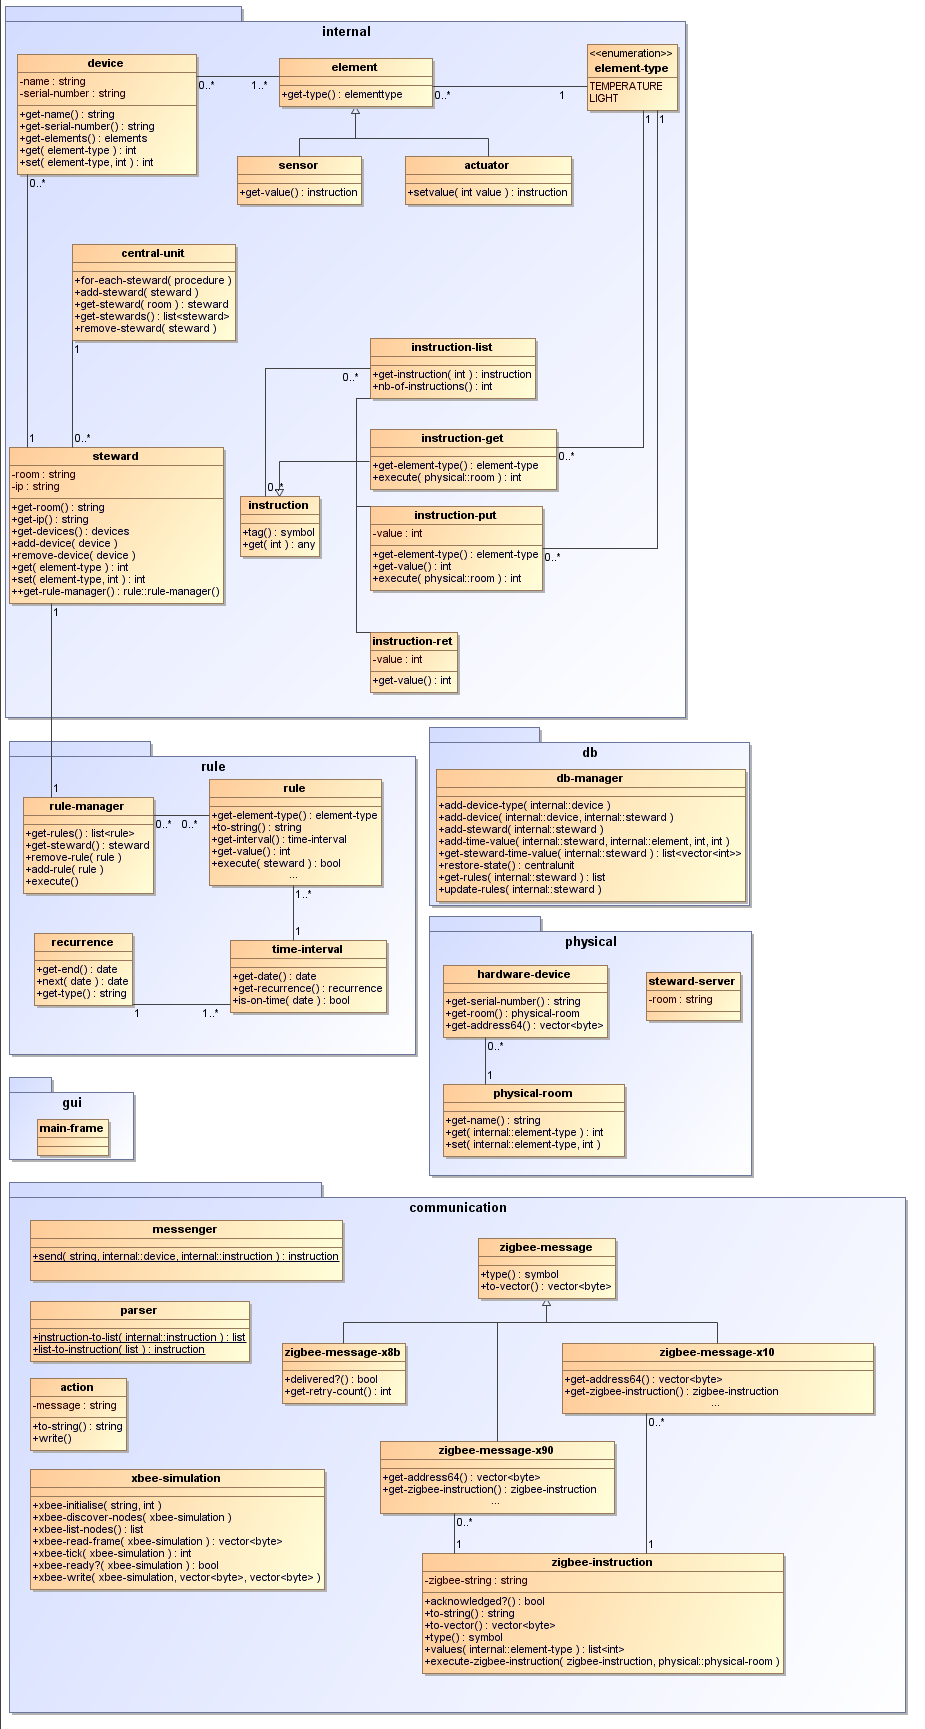
\includegraphics[width=\columnwidth]{class-diagram/class-diagram.png}}
	\end{center}
	\caption{Het class-diagram}
\end{figure}

\newpage
\hypertarget{internal}{\section{internal}}
\label{internal}
Het internal module bevat de kern van het domotica systeem. De central-unit houdt de verschillende stewards bij, die instructies kunnen zenden aan de hardware, zoals het aanpassen van de licht-intensiteit of het opvragen van de temperatuur van de kamer.

\subsection{Overview}

\subsubsection{Class}
\begin{description}
\item[\hyperlink{element}{element}] : Een abstacte classe die een bepaalde element-type bijhoud.
\item[\hyperlink{sensor}{sensor}] : Vraagt informatie over zijn element-type op.
\item[\hyperlink{actuator}{actuator}] : Laat toe om de informatie van zijn element-type aan te passen.
\item[\hyperlink{device}{device}] : Een toestel die een aantal sensoren en activatoren bevat.
\item[\hyperlink{steward}{steward}] : Bevat en beheerst een aantal devices.
\item[\hyperlink{central-unit}{central-unit}] : Bevat een aantal stewards.
\item[\hyperlink{instruction}{instruction}] : Een instructie die naar de hardware verzonden kan worden.
\item[\hyperlink{instruction-get}{instruction-get}] : Instructie om een element-type te krijgen.
\item[\hyperlink{instruction-put}{instruction-put}] : Instructie om een element-type aan te passen.
\item[\hyperlink{instruction-list}{instruction-list}] : Een lijst van instructions.
\item[\hyperlink{instruction-ret}{instruction-ret}] : Een return instructie die een waarde teruggeeft.
\end{description}

\subsubsection{Enum}
\begin{description}
\item[\hyperlink{element-type}{element-type}] : Alle mogelijke types elementen die door de applicatie toegelaten zijn.
\end{description}

\newpage
%\subsubsection{element-type}
\hypertarget{element-type}{\subsection{element-type}}
Alle mogelijke types elementen die door de applicatie toegelaten zijn. element-type representeert de verschillende attributen die meetbaar zijn door sensoren en aanpasbaar door actuatoren.

\subsubsection{Value}
\begin{description}
\item[\racket{\code{TEMPERATURE}}] : Temperatuur.
\item[\racket{\code{LIGHT}}] : Licht-intensiteit.
\end{description}

\subsubsection{Method}
\begin{description}
\item[\hyperlink{element-type:to-string}{\racket{\lb[to-string] element-type\rb \ar \code{string?}}}] : Zet een element-type om naar een string.
\item[\hyperlink{element-type:for-each-element-type}{\racket{\lb[for-each-element-type] proc\rb \ar \code{void?}}}] : Past de procedure proc toe voor elk element-type.
\end{description}

\begin{framed}
%(to-string element-type) -> string?
\hypertarget{element-type:to-string}{\racket{\lb[to-string] element-type\rb \ar \code{string?}}}
\\Zet een element-type om naar een string.
\begin{itemize}
	\item \emph{element-type} : het type dat omgezet moet worden.
	\item \emph{return} : de resulterende string.
\end{itemize}
\end{framed}

\begin{framed}
%(for-each-element-type proc) -> void?
\hypertarget{element-type:for-each-element-type}{\racket{\lb[for-each-element-type] proc\rb \ar \code{void?}}}
\\Past de procedure proc toe voor elk element-type.
\begin{itemize}
	\item \emph{proc} : de procedure die op elk element-type moet toegepast worden.
\end{itemize}
\end{framed}

\newpage
\hypertarget{element}{\subsection{element}}
Een abstacte classe die een bepaalde element-type bijhoud.
\\\textbf{Known Implementations :} \hyperlink{sensor}{sensor}, \hyperlink{actuator}{actuator}.

\subsubsection{Constructor}
\begin{description}
\item[\hyperlink{element:new-element}{\racket{\lb[new-element] element-type\rb \ar \code{procedure?}}}] : Maakt een nieuw element aan.
\end{description}

\subsubsection{Method}
\begin{description}
\item[\hyperlink{element:class}{\racket{\lb[class]\rb \ar \code{symbol?}}}] : Geeft de naam van de classe terug.
\item[\hyperlink{element:get-type}{\racket{\lb[get-type]\rb \ar \code{element-type?}}}] : Geeft het type element van dit element.
\end{description}

\begin{framed}
\hypertarget{element:new-element}{\racket{\lb[new-element] element-type\rb \ar \code{procedure?}}}
\\Maakt een nieuw element aan van een bepaalde element-type.
\begin{itemize}
	\item \emph{element-type} : Het type van dit element.
\end{itemize}
\end{framed}

\begin{framed}
\hypertarget{element:class}{\racket{\lb[class]\rb \ar \code{symbol?}}}
\\Geeft de naam van de classe terug, in dit geval \racket{Element}.
\begin{itemize}
	\item \emph{return} : De naam van de classe.
\end{itemize}
\end{framed}

\begin{framed}
\hypertarget{element:get-type}{\racket{\lb[get-type]\rb \ar \code{element-type?}}}
\\Geeft het type element van dit element.
\begin{itemize}
	\item \emph{return} : Het element-type.
\end{itemize}
\end{framed}

\newpage
\hypertarget{sensor}{\subsection{sensor}}
Vraagt informatie over zijn element-type op. Een sensor genereert een instruction die de waarde van zijn element-type opvraagt. Deze instruction kan daarna via een messenger verzonden worden naar hardware zodat die het element-type meet.
\\\textbf{Inherit :} \hyperlink{element}{element}.

\subsubsection{Constructor}
\begin{description}
\item[\hyperlink{sensor:new-sensor}{\racket{\lb[new-sensor] element-type\rb \ar \code{procedure?}}}] : Maakt een nieuwe sensor aan.
\end{description}

\subsubsection{Method}
\begin{description}
\item[\hyperlink{sensor:class}{\racket{\lb[class]\rb \ar \code{symbol?}}}] : Geeft de naam van de classe terug.
\item[\hyperlink{sensor:super}{\racket{\lb[super]\rb \ar \code{element?}}}] : Geeft de instantie van de superclasse van het sensor-object.
\item[\hyperlink{sensor:get-value}{\racket{\lb[get-value]\rb \ar \code{instruction?}}}] : Vraagt de waarde van deze sensor's element-type.
\end{description}

\begin{framed}
\hypertarget{sensor:new-sensor}{\racket{\lb[new-sensor] element-type\rb \ar \code{procedure?}}}
\\Maakt een nieuwe sensor aan.
\begin{itemize}
	\item \emph{element-type} : Het type van deze sensor.
\end{itemize}
\end{framed}

\begin{framed}
\hypertarget{sensor:class}{\racket{\lb[class]\rb \ar \code{symbol?}}}
\\Geeft de naam van de classe terug, in dit geval \racket{Sensor}.
\begin{itemize}
	\item \emph{return} : De naam van de classe.
\end{itemize}
\end{framed}

\begin{framed}
\hypertarget{sensor:super}{\racket{\lb[super]\rb \ar \code{element?}}}
\\Geeft de instantie van de superclasse van het sensor-object.
\begin{itemize}
	\item \emph{return} : Het superclasse object.
\end{itemize}
\end{framed}

\begin{framed}
\hypertarget{sensor:get-value}{\racket{\lb[get-value]\rb \ar \code{instruction?}}}
\\Deze procedure genereert een \racket{instruction-get} die verzonden kan worden naar hardware zodat deze de waarde opvraagt van deze sensor's element-type in de kamer waarin die zich bevindt.
\begin{itemize}
	\item \emph{return} : De antwoord-instructie.
\end{itemize}
\end{framed}

\newpage
\hypertarget{actuator}{\subsection{actuator}}
Laat toe om de informatie van zijn element-type aan te passen. Een actuator genereert een instruction die later verzonden kan worden naar de hardware. Deze instruction past de waarde van element-type naar een nieuwe waarde toe.
\\\textbf{Inherit :} \hyperlink{element}{element}.

\subsubsection{Constructor}
\begin{description}
\item[\hyperlink{actuator:new-actuator}{\racket{\lb[new-actuator] element-type\rb \ar \code{procedure?}}}] : Maakt een nieuwe actuator aan.
\end{description}

\subsubsection{Method}
\begin{description}
\item[\hyperlink{actuator:class}{\racket{\lb[class]\rb \ar \code{symbol?}}}] : Geeft de naam van de classe terug.
\item[\hyperlink{actuator:super}{\racket{\lb[super]\rb \ar \code{element?}}}] : Geeft de instantie van de superclasse van het actuator-object.
\item[\hyperlink{actuator:set-value}{\racket{\lb[set-value] value\rb \ar \code{instruction?}}}] : Past de waarde van deze actuator aan.
\end{description}

\begin{framed}
\hypertarget{actuator:new-actuator}{\racket{\lb[new-actuator] element-type\rb \ar \code{procedure?}}}
\\Maakt een nieuwe actuator aan.
\begin{itemize}
	\item \emph{element-type} : Het type van deze actuator.
\end{itemize}
\end{framed}

\begin{framed}
\hypertarget{actuator:class}{\racket{\lb[class]\rb \ar \code{symbol?}}}
\\Geeft de naam van de classe terug, in dit geval \racket{Actuator}.
\begin{itemize}
	\item \emph{return} : De naam van de classe.
\end{itemize}
\end{framed}

\begin{framed}
\hypertarget{actuator:super}{\racket{\lb[super]\rb \ar \code{element?}}}
\\Geeft de instantie van de superclasse van het actuator-object.
\begin{itemize}
	\item \emph{return} : Het superclasse object.
\end{itemize}
\end{framed}

\begin{framed}
\hypertarget{actuator:set-value}{\racket{\lb[set-value] value\rb \ar \code{instruction?}}}
\\Deze procedure genereert een \racket{instruction-put} die vraagt om de waarde van deze actuator's element-type aan te passen naar value.
\begin{itemize}
	\item \emph{value} : De nieuwe waarde.
	\item \emph{return} : De antwoord-instructie.
\end{itemize}
\end{framed}

\newpage
\hypertarget{device}{\subsection{device}}
Een toestel die een aantal sensoren en actuatoren bevat. Een device kan de element-types van de kamer waarin hij zich bevindt opvragen en aanpassen, vermits hij bestaat uit de corresponderende sensoren en actuatoren.

\subsubsection{Constructor}
\begin{description}
\item[\hyperlink{device:new-device}{\racket{\lb[new-device] name serial-number\rb \ar \code{procedure?}}}] : Maakt een nieuwe device aan.
\end{description}

\subsubsection{Method}
\begin{description}
\item[\hyperlink{device:class}{\racket{\lb[class]\rb \ar \code{symbol?}}}] : Geeft de naam van de classe terug.
\item[\hyperlink{device:get-name}{\racket{\lb[get-name]\rb \ar \code{string?}}}] : De naam van deze device.
\item[\hyperlink{device:get-serial-number}{\racket{\lb[get-serial-number]\rb \ar \code{string?}}}] : Het serial-nummer van deze device.
\item[\hyperlink{device:get-elements}{\racket{\lb[get-elements]\rb \ar \lb[listof] element?\rb}}] : Een lijst van de elements die de device bevat.
\item[\hyperlink{device:add-element}{\racket{\lb[add-element] element\rb \ar \code{void?}}}] : Voeg een element toe aan de device.
\item[\hyperlink{device:get}{\racket{\lb[get] element-type\rb \ar \lb[or/c] \#f number?\rb}}] : Vraagt informatie over het meegegeefde element-type.
\item[\hyperlink{device:set}{\racket{\lb[set] element-type value\rb \ar \lb[or/c] \#f number?\rb}}] : Past element-type naar value aan.
\end{description}

\begin{framed}
\hypertarget{device:new-device}{\racket{\lb[new-device] name serial-number\rb \ar \code{procedure?}}}
\\Maakt een nieuwe device aan. Deze device heeft een naam en een uniek serial-number. Alle devices met dezelfde naam hebben ook dezelfde sensoren en actuatoren (ze hebben wel een verschillend serial-number).
\\Stel we hebben een device "thermostat" die een \racket{TEMPERATURE} sensor en actuator heeft, dan hebben nieuwe devices met de naam "thermostat" ook deze sensor en actuator.
\begin{itemize}
	\item \emph{name} : De naam van de device.
	\item \emph{serial-number} : Het unieke serial-nummer van de device.
\end{itemize}
\end{framed}

\begin{framed}
\hypertarget{device:class}{\racket{\lb[class]\rb \ar \code{symbol?}}}
\\Geeft de naam van de classe terug, in dit geval \racket{Device}.
\begin{itemize}
	\item \emph{return} : De naam van de classe.
\end{itemize}
\end{framed}

\begin{framed}
\hypertarget{device:get-name}{\racket{\lb[get-name]\rb \ar \code{string?}}}
\\De naam van deze device.
\begin{itemize}
	\item \emph{return} : De naam.
\end{itemize}
\end{framed}

\begin{framed}
\hypertarget{device:get-serial-number}{\racket{\lb[get-serial-number]\rb \ar \code{string?}}}
\\Het unieke serial-nummer van deze device.
\begin{itemize}
	\item \emph{return} : Het serial-nummer.
\end{itemize}
\end{framed}

\begin{framed}
\hypertarget{device:get-elements}{\racket{\lb[get-elements]\rb \ar \lb[listof] element?\rb}}
\\Een lijst van de verschillende sensoren en actuatoren waaruit deze device bestaat.
\begin{itemize}
	\item \emph{return} : De lijst van elements.
\end{itemize}
\end{framed}

\begin{framed}
\hypertarget{device:add-element}{\racket{\lb[add-element] element\rb \ar \code{void?}}}
\\Voegt een nieuw element toe aan deze device.
\begin{itemize}
	\item \emph{element} : Het element dat toegevoegd moet worden.
\end{itemize}
\end{framed}

\begin{framed}
\hypertarget{device:get}{\racket{\lb[get] element-type\rb \ar \lb[or/c] \#f number?\rb}}
\\Vraagt informatie over het meegegeefde element-type. De device zoekt of het een sensor heeft met het gevraagde element-type. Het gebruikt dan die sensor om een instruction te genereren die hij gaat zenden naar zijn corresponderen hardware via de messenger. De hardware voert de instructie uit en zendt het antwoord terug naar deze device, die daaruit het resultaat ophaalt en teruggeeft.
\begin{itemize}
	\item \emph{element-type} : Het type dat gevraagd wordt.
	\item \emph{return} : \racket{\#f} wanneer de informatie niet gevraagd kon worden (wegens het mankeren van de sensor voor dit soort element-type).\\\racket{number?} De waarde van het element-type.
\end{itemize}
\end{framed}

\begin{framed}
\hypertarget{device:set}{\racket{\lb[set] element-type value\rb \ar \lb[or/c] \#f number?\rb}}
\\Past element-type naar value aan. De device zoekt naar een actuator met het gevraagde element-type. Deze actuator wordt dan gebruikt om een instruction te genereren. Die instruction wordt via de messenger verzonden naar deze device's corresponderende hardware. Na het uitvoeren van de instructie wordt het antwoord terugverzonden.
\begin{itemize}
	\item \emph{element-type} : Het type dat aangepast moet worden.
	\item \emph{value} : De nieuwe waarde van het type.
	\item \emph{return} : \racket{\#f} wanneer de informatie niet aangepast kon worden (wegens het mankeren van een actuator voor dit soort element-type).\\\racket{number?} Een bewijs dat de informatie aangepast is.
\end{itemize}
\end{framed}

\newpage
\hypertarget{steward}{\subsection{steward}}
Bevat en beheert een aantal devices. De steward kan aan devices vragen om de element-types van de room waarin hij zich bevindt op te vragen en aanpassen (vermits hij de nodige device heeft).

\subsubsection{Constructor}
\begin{description}
	\item[\hyperlink{steward:new-steward}{\racket{\lb[new-steward] room\rb \ar \code{procedure?}}}] : Maakt een nieuwe steward aan.
\end{description}

\subsubsection{Method}
\begin{description}
	\item[\hyperlink{steward:class}{\racket{\lb[class]\rb \ar \code{symbol?}}}] : Geeft de naam van de classe terug.
	\item[\hyperlink{steward:get-room}{\racket{\lb[get-room]\rb \ar \code{string?}}}] : De kamer waarin deze steward ligt.
	\item[\hyperlink{steward:get-devices}{\racket{\lb[get-devices]\rb \ar \lb[listof] device?\rb}}] : Een lijst van de devices die deze steward beheert.
	\item[\hyperlink{steward:add-device}{\racket{\lb[add-device] device\rb \ar \code{void?}}}] : Voeg een device toe aan deze steward.
	\item[\hyperlink{steward:get}{\racket{\lb[get] element-type\rb \ar \lb[or/c] \#f number?\rb}}] : Vraagt informatie over het meegegeevde element-type.
	\item[\hyperlink{steward:set}{\racket{\lb[set] element-type value\rb \ar \lb[or/c] \#f number?\rb}}] : Past het element-type naar value aan.
\end{description}

\begin{framed}
\hypertarget{steward:new-steward}{\racket{\lb[new-steward] room\rb \ar \code{procedure?}}}
\\Maakt een nieuwe steward aan, er kan maar een steward per kamer zijn, elke room moet dus uniek zijn.
\begin{itemize}
	\item \emph{room} : De kamer waarin deze steward ligt.
\end{itemize}
\end{framed}	

\begin{framed}
\hypertarget{steward:class}{\racket{\lb[class]\rb \ar \code{symbol?}}}
\\Geeft de naam van de classe terug, in dit geval \racket{Steward}.
\begin{itemize}
	\item \emph{return} : De naam van de classe.
\end{itemize}
\end{framed}

\begin{framed}
\hypertarget{steward:get-room}{\racket{\lb[get-room]\rb \ar \code{string?}}}
\\De kamer waarin deze steward ligt.
\begin{itemize}
	\item \emph{return} : De kamer.
\end{itemize}
\end{framed}

\begin{framed}
\hypertarget{steward:get-devices}{\racket{\lb[get-devices]\rb \ar \lb[listof] device?\rb}}
\\Een lijst van de devices die deze steward beheert.
\begin{itemize}
	\item \emph{return} : De lijst van devices.
\end{itemize}
\end{framed}

\begin{framed}
\hypertarget{steward:add-device}{\racket{\lb[add-device] device\rb \ar \code{void?}}}
\\Voeg een device toe aan deze steward. Elke device kan maar van een steward afhangen.
\begin{itemize}
	\item \emph{device} : De device die toegevoegd wordt.
\end{itemize}
\end{framed}

\begin{framed}
\hypertarget{steward:get}{\racket{\lb[get] element-type\rb \ar \lb[or/c] \#f number?\rb}}
\\Vraagt informatie over het meegegeefde element-type. De steward zoekt naar een sensor van het gevraagde type in de lijst van devices die hij beheert. Een instructie wordt dan verzonden naar de hardware om informatie te krijgen over het type in de kamer van de steward.
\begin{itemize}
	\item \emph{element-type} : Het gevraagde type.
	\item \emph{return} : \racket{\#f} als er geen sensor is voor het gezochte element-type.\\\racket{number?} De gevraagde informatie.
\end{itemize}
\end{framed}

\begin{framed}
\hypertarget{steward:set}{\racket{\lb[set] element-type value\rb \ar \lb[or/c] \#f number?\rb}}
\\Past het element-type naar value aan. De steward zoekt naar een actuator in zijn lijst van devices die element-type zou kunnen aanpassen. Informatie wordt dan verzonden naar de hardware om element-type in de kamer van de steward te veranderen.
\begin{itemize}
	\item \emph{element-type} : Het type dat aangepast moet worden.
	\item \emph{value} : De waarde waarop het type gezet moet worden.
	\item \emph{return} : \racket{\#f} als er geen actuator is voor het gezochte element-type.\\\racket{number?} Een bewijs dat element-type aangepast werd.
\end{itemize}
\end{framed}

\newpage
\hypertarget{central-unit}{\subsection{central-unit}}
Bevat een aantal stewards.

\subsubsection{Constructor}
\begin{description}
	\item[\hyperlink{central-unit:new-central-unit}{\racket{\lb[new-central-unit]\rb \ar \code{procedure?}}}] : Maakt een nieuwe central-unit aan.
\end{description}

\subsubsection{Method}
\begin{description}
	\item[\hyperlink{central-unit:class}{\racket{\lb[class]\rb \ar \code{symbol?}}}] : Geeft de naam van de classe terug.
	\item[\hyperlink{central-unit:for-each-steward}{\racket{\lb[for-each-steward] proc\rb \ar \code{void?}}}] : Past de procedure proc toe voor elke steward die de central-unit beheert.
	\item[\hyperlink{central-unit:add-steward}{\racket{\lb[add-steward] steward\rb \ar \code{void?}}}] : Voegt een nieuwe steward toe.
	\item[\hyperlink{central-unit:get-steward}{\racket{\lb[get-steward] room\rb \ar \code{steward?}}}] : Zoekt voor een bepaalde steward in de lijst van stewards van de central-unit.
\end{description}

\begin{framed}
	\hypertarget{central-unit:new-central-unit}{\racket{\lb[new-central-unit]\rb \ar \code{procedure?}}}
	\\Maakt een nieuwe central-unit aan.
\end{framed}

\begin{framed}
	\hypertarget{central-unit:class}{\racket{\lb[class]\rb \ar \code{symbol?}}}
	\\Geeft de naam van de classe terug, in dit geval \racket{CentralUnit}.
	\begin{itemize}
		\item \emph{return} : De naam van de classe.
	\end{itemize}
\end{framed}

\begin{framed}
	\hypertarget{central-unit:for-each-steward}{\racket{\lb[for-each-steward] proc\rb \ar \code{void?}}}
	\\Past de procedure proc toe voor elke steward die de central-unit beheert.
	\begin{itemize}
		\item \emph{proc} : De procedure die op elke steward toegepast wordt.
	\end{itemize}
\end{framed}

\begin{framed}
	\hypertarget{central-unit:add-steward}{\racket{\lb[add-steward] steward\rb \ar \code{void?}}}
	\\Voegt een nieuwe steward toe.
	\begin{itemize}
		\item \emph{steward} : De steward die toegevoegd moet worden.
	\end{itemize}
\end{framed}

\begin{framed}
	\hypertarget{central-unit:get-steward}{\racket{\lb[get-steward] room\rb \ar \code{steward?}}}
	\\Zoekt voor een bepaalde steward in de lijst van stewards van de central-unit.
	\begin{itemize}
		\item \emph{room} : The kamer waarin de steward is (het room-attribuut van de gezochte steward).
		\item \emph{return} : De gevonden steward.
	\end{itemize}
\end{framed}

\newpage
\hypertarget{instruction}{\subsection{instruction}}
Een instructie die naar de hardware verzonden kan worden.
\\\textbf{Known Implementations :} \hyperlink{instruction-get}{instruction-get}, \hyperlink{instruction-put}{instruction-put}, \hyperlink{instruction-list}{instruction-list}, \hyperlink{instruction-ret}{instruction-ret}.

\subsubsection{Constructor}
\begin{description}
	\item[\hyperlink{instruction:new-instruction}{\racket{\lb[new-instruction] tag . args\rb \ar \code{procedure?}}}] : Maakt een nieuwe instruction aan.
\end{description}

\subsubsection{Method}
\begin{description}
	\item[\hyperlink{instruction:tag}{\racket{\lb[tag]\rb \ar \code{symbol?}}}] : Geeft de tag terug van deze instruction.
	\item[\hyperlink{instruction:get}{\racket{\lb[get] i\rb \ar \code{any?}}}] : Geeft het i-de argument van de instruction terug.
\end{description}

\begin{framed}
	\hypertarget{instruction:new-instruction}{\racket{\lb[new-instruction] tag . args\rb \ar \code{procedure?}}}
	\\Maakt een nieuwe instruction aan.
	\begin{itemize}
		\item \emph{tag} : De tag dat deze instruction definieerd.
		\item \emph{args} : de verschillende argumenten dat aan deze instructie meegegeven worden.
	\end{itemize}
\end{framed}

\begin{framed}
	\hypertarget{instruction:tag}{\racket{\lb[tag]\rb \ar \code{symbol?}}}
	\\Geeft de tag terug van deze instruction.
	\begin{itemize}
		\item \emph{return} : De tag dat deze instruction definieerd.
	\end{itemize}
\end{framed}

\begin{framed}
	\hypertarget{instruction:get}{\racket{\lb[get] i\rb \ar \code{any?}}}
	\\Geeft het i-de argument van de instruction terug.
	\begin{itemize}
		\item \emph{i} : De positie van het gezochte argument.
		\item \emph{return} : Het i-de argument.
	\end{itemize}
\end{framed}

\newpage
\hypertarget{instruction-get}{\subsection{instruction-get}}
Instructie om een element-type te krijgen. Wanneer die verzonden wordt naar de hardware gaat deze instructie de waarde van het element-type opvragen (in de kamer waar de hardware zich bevindt).
\\\textbf{Inherit} : \hyperlink{instruction}{instruction}.

\subsubsection{Constructor}
\begin{description}
	\item[\hyperlink{instruction-get:new-instruction-get}{\racket{\lb[new-instruction-get] element-type\rb \ar \code{procedure?}}}] : Maakt een nieuwe instruction-get aan.
\end{description}

\subsubsection{Method}
\begin{description}
	\item[\hyperlink{instruction-get:tag}{\racket{\lb[tag]\rb \ar \code{symbol?}}}] : Geeft de tag \racket{TAG\_GET} terug.
	\item[\hyperlink{instruction-get:get-element-type}{\racket{\lb[get-element-type]\rb \ar \code{element-type?}}}] : Geeft het element-type van deze instruction terug.
	\item[\hyperlink{instruction-get:execute}{\racket{\lb[execute] room\rb \ar \code{number?}}}] : Geeft de waarde van de instruction-get's element-type voor deze room.
\end{description}

\begin{framed}
	\hypertarget{instruction-get:new-instruction-get}{\racket{\lb[new-instruction-get] element-type\rb \ar \code{procedure?}}}
	\\Maakt een nieuwe instruction-get aan.
	\begin{itemize}
		\item \emph{element-type} : De type van deze instruction-get.
	\end{itemize}
\end{framed}

\begin{framed}
	\hypertarget{instruction-get:tag}{\racket{\lb[tag]\rb \ar \code{symbol?}}}
	\\Geeft de tag \racket{TAG\_GET} terug.
	\begin{itemize}
		\item \emph{return} : \racket{TAG\_GET}
	\end{itemize}
\end{framed}

\begin{framed}
	\hypertarget{instruction-get:get-element-type}{\racket{\lb[get-element-type]\rb \ar \code{element-type?}}}
	\\Geeft het element-type van deze instruction terug.
	\begin{itemize}
		\item \emph{return} : Het element-type van deze instruction-get.
	\end{itemize}
\end{framed}

\begin{framed}
	\hypertarget{instruction-get:execute}{\racket{\lb[execute] room\rb \ar \code{number?}}}
	\\Geeft de waarde van de instruction-get's element-type voor deze room.
	\begin{itemize}
		\item \emph{room} : De kamer waarvan we de element-type willen weten.
		\item \emph{return} : de waarde van element-type in room.
	\end{itemize}
\end{framed}

\newpage
\hypertarget{instruction-put}{\subsection{instruction-put}}
Instructie om een element-type aan te passen. Wanneer die verzonden wordt naar hardware gaat die de waarde van zijn element-type aanpassen (in de room waar de hardware zich bevindt).

\subsubsection{Constructor}
\begin{description}
	\item[\hyperlink{instruction-put:new-instruction-put}{\racket{\lb[new-instruction-put] element-type value\rb \ar \code{procedure?}}}] : Maakt een nieuwe instruction-put aan.
\end{description}

\subsubsection{Method}
\begin{description}
	\item[\hyperlink{instruction-put:tag}{\racket{\lb[tag]\rb \ar \code{symbol?}}}] : Geeft de tag \racket{TAG\_PUT} terug.
	\item[\hyperlink{instruction-put:get-element-type}{\racket{\lb[get-element-type]\rb \ar \code{element-type?}}}] : Geeft het element-type van deze instruction terug.
	\item[\hyperlink{instruction-put:get-value}{\racket{\lb[get-value]\rb \ar \code{number?}}}] : Geeft de waarde van deze instruction-put terug.
	\item[\hyperlink{instruction-put:execute}{\racket{\lb[execute] room\rb \ar \code{number?}}}] : Past de waarde van deze instruction's element-type aan naar een nieuwe waarde in room.
\end{description}	

\begin{framed}
	\hypertarget{instruction-put:new-instruction-put}{\racket{\lb[new-instruction-put] element-type value\rb \ar \code{procedure?}}}
	\\Maakt een nieuwe instruction-put aan.
	\begin{itemize}
		\item \emph{element-type} : De element-type van deze instruction.
		\item \emph{value} : De waarde die deze instruction gaat zetten bij het aanpassen van element-type.
	\end{itemize}
\end{framed}

\begin{framed}
	\hypertarget{instruction-put:tag}{\racket{\lb[tag]\rb \ar \code{symbol?}}}
	\\Geeft de tag \racket{TAG\_PUT} terug.
	\begin{itemize}
		\item \emph{return} : \racket{TAG\_PUT}.
	\end{itemize}
\end{framed}

\begin{framed}
	\hypertarget{instruction-put:get-element-type}{\racket{\lb[get-element-type]\rb \ar \code{element-type?}}}
	\\Geeft het element-type van deze instruction terug.
	\begin{itemize}
		\item \emph{return} : Het element-type van deze instruction-put.
	\end{itemize}
\end{framed}

\begin{framed}
	\hypertarget{instruction-put:get-value}{\racket{\lb[get-value]\rb \ar \code{number?}}}
	\\Geeft de waarde van deze instruction-put terug.
	\begin{itemize}
		\item \emph{return} : De waarde van deze instruction.
	\end{itemize}
\end{framed}

\begin{framed}
	\hypertarget{instruction-put:execute}{\racket{\lb[execute] room\rb \ar \code{number?}}}
	\\Past de waarde van deze instruction's element-type aan naar een nieuwe waarde in room.
	\begin{itemize}
		\item \emph{room} : De kamer waarin de element-type aangepast zal worden.
		\item \emph{return} : De aangepaste waarde van de kamer.
	\end{itemize}
\end{framed}

\newpage
\hypertarget{instruction-list}{\subsection{instruction-list}}
Een lijst van instructions.
\\\textbf{Inherit} : \hyperlink{instruction}{instruction}

\subsubsection{Constructor}
\begin{description}
	\item[\hyperlink{instruction-list:new-instruction-list}{\racket{\lb[new-instruction-list] . instructions\rb \ar \code{procedure?}}}] : Maakt een nieuwe instruction-list aan.
\end{description}

\subsubsection{Method}
\begin{description}
	\item[\hyperlink{instruction-list:tag}{\racket{\lb[tag]\rb \ar \code{symbol?}}}] : Geeft de tag \racket{TAG\_LIST} terug.
	\item[\hyperlink{instruction-list:get-instruction}{\racket{\lb[get-instruction] i\rb \ar \code{instruction?}}}] : Geeft de i-de instruction terug.
	\item[\hyperlink{instruction-list:nb-of-instructions}{\racket{\lb[nb-of-instructions]\rb \ar \code{number?}}}] : Geeft het aantal instructions die deze instruction-list bevat.
\end{description}

\begin{framed}
	\hypertarget{instruction-list:new-instruction-list}{\racket{\lb[new-instruction-list] . instructions\rb \ar \code{procedure?}}}
	\\Maakt een nieuwe instruction-list aan.
	\begin{itemize}
		\item \emph{instructions} : De instructions die deze lijst bevat.
	\end{itemize}
\end{framed}

\begin{framed}
	\hypertarget{instruction-list:tag}{\racket{\lb[tag]\rb \ar \code{symbol?}}}
	\\Geeft de tag \racket{TAG\_LIST} terug.
	\begin{itemize}
		\item \emph{return} : \racket{TAG\_LIST}.
	\end{itemize}
\end{framed}

\begin{framed}
	\hypertarget{instruction-list:get-instruction}{\racket{\lb[get-instruction] i\rb \ar \code{instruction?}}}
	\\Geeft de i-de instruction terug.
	\begin{itemize}
		\item \emph{i} : De positie van de gezochte instruction.
		\item \emph{return} : De instruction op positie i.
	\end{itemize}
\end{framed}	

\begin{framed}
	\hypertarget{instruction-list:nb-of-instructions}{\racket{\lb[nb-of-instructions]\rb \ar \code{number?}}}
	\\Geeft het aantal instructions die deze instruction-list bevat.
	\begin{itemize}
		\item \emph{return} : Het aantal instructions die deze lijst bevat.
	\end{itemize}
\end{framed}

\newpage
\hypertarget{instruction-ret}{\subsection{instruction-ret}}
Een return instructie die een waarde teruggeeft. Deze instructions worden door de hardware als antwoord gegenereerd naar het uitvoeren van een instruction-get of -put.
\textbf{Inherit} : \hyperlink{instruction}{instruction}

\subsubsection{Constructor}
\begin{description}
	\item[\hyperlink{instruction-ret:new-instruction-ret}{\racket{\lb[new-instruction-ret] value\rb \ar \code{procedure?}}}] : Maakt een nieuwe instruction-ret aan.
\end{description}

\subsubsection{Method}
\begin{description}
	\item[\hyperlink{instruction-ret:tag}{\racket{\lb[tag]\rb \ar \code{symbol?}}}] : Geeft de tag \racket{TAG\_RET} terug.
	\item[\hyperlink{instruction-ret:get-value}{\racket{\lb[get-value]\rb \ar \code{number?}}}] : Geeft de waarde van deze instruction terug.
\end{description}

\begin{framed}
	\hypertarget{instruction-ret:new-instruction-ret}{\racket{\lb[new-instruction-ret] value\rb \ar \code{procedure?}}}
	\\Maakt een nieuwe instruction-ret aan.
	\begin{itemize}
		\item \emph{value} : De waarde van deze instruction-ret.
	\end{itemize}
\end{framed}

\begin{framed}
	\hypertarget{instruction-ret:tag}{\racket{\lb[tag]\rb \ar \code{symbol?}}}
	\\Geeft de tag \racket{TAG\_RET} terug.
	\begin{itemize}
		\item \emph{return} : \racket{TAG\_RET}.
	\end{itemize}
\end{framed}

\begin{framed}
	\hypertarget{instruction-ret:get-value}{\racket{\lb[get-value]\rb \ar \code{number?}}}
	\\Geeft de waarde van deze instruction terug.
	\begin{itemize}
		\item \emph{return} : De waarde.
	\end{itemize}
\end{framed}

\newpage
\hypertarget{communication}{\section{communication}}
Laat toe om boodschappen te sturen naar de hardware. Dit module bevat het nodige om te communiceren tussen de steward en de hardware door het zenden en opvangen van instructions.

\subsection{Overview}

\subsubsection{Class}
	\begin{description}
		\item[\hyperlink{messenger}{messenger}] : Kan instructions sturen naar de hardware via ports.
		\item[\hyperlink{parser}{parser}] : Zet een instruction om naar een lijst van symbols en omgekeerd.
	\end{description}
	
	\newpage
	\hypertarget{messenger}{\subsection{messenger}}
	Kan instructions sturen naar de hardware via ports. Wanneer een device een instruction wilt zenden zoekt de messenger naar de port waar de corresponderende hardware-device naar luisterd. De instruction wordt dan geparsed en verzonden. Een antwoord wordt door de hardware-device gestuurd.
	\subsubsection{Method}
	\begin{description}
		\item[\hyperlink{messenger:send}{\racket{\lb[send] device instruction\rb \ar \code{instruction?}}}] : Zendt een instruction naar een bepaalde device.
	\end{description}
	
	\begin{framed}
		\hypertarget{messenger:send}{\racket{\lb[send] device instruction\rb \ar \code{instruction?}}}
		\\Zendt een instruction naar een bepaalde device.
		\begin{itemize}
			\item \emph{device} : De messenger zoekt naar de port van de corresponderende hardware-device. Daar zal de instruction verzonden worden.
			\item \emph{instruction} : De instruction die verzonden moet worden.
			\item \emph{return} : Een antwoord instruction.
		\end{itemize}
	\end{framed}
	
	\newpage
	\hypertarget{parser}{\subsection{parser}}
	De parser zet een instruction om naar een lijst zodat die via ports gestuurd kan worden.  Deze zorgt ook voor het terug-omzetten van lijsten naar geldige instructions.
	
	\subsubsection{Method}
		\begin{description}
			\item[\hyperlink{parser:instruction-to-list}{\racket{\lb[instruction-to-list] instruction\rb \ar \lb[listof] symbol?\rb}}] : Zet een instruction om naar een list.
			\item[\hyperlink{parser:list-to-instruction}{\racket{\lb[list-to-instruction] lst\rb \ar \code{instruction?}}}] : Zet een list om naar een instruction.
		\end{description}
		
		\begin{framed}
			\hypertarget{parser:instruction-to-list}{\racket{\lb[instruction-to-list] instruction\rb \ar \lb[listof] symbol?\rb}}
			\\Zet een instruction om naar een list.
			\begin{itemize}
				\item \emph{instruction} : De instruction dat omgezet moet worden.
				\item \emph{return} : Een lijst die de instruction voorstelt.
			\end{itemize}
		\end{framed}
		
		\begin{framed}
			\hypertarget{parser:list-to-instruction}{\racket{\lb[list-to-instruction] lst\rb \ar \code{instruction?}}}
			\\Zet een lijst om naar een instruction.
			\begin{itemize}
				\item \emph{lst} : De lijst de naar een instruction omgezet moet worden.
				\item \emph{return} : De instruction die de lijst representeerde.
			\end{itemize}
		\end{framed}
		
\newpage
\hypertarget{physical}{\section{physical}}
Omdat we nog niet met hardware omgaan wordt deze gesimuleerd. 

\subsection{Overview}

\subsubsection{Class}
\begin{description}
		\item[\hyperlink{hardware-device}{hardware-device}] : Simuleert het gedrag van hardware devices (zoals een thermostaat).
		\item[\hyperlink{physical-room}{physical-room}] : De gesimuleerde hardware bevindt zich in een kamer, dit wordt gesimuleert door physical-room.
\end{description}

\newpage
\hypertarget{hardware-device}{\subsection{hardware-device}}
Simuleert het gedrag van hardware devices (zoals een thermostaat). Een hardware-device luistert naar een bepaalde port en voert instructions uit die door die port verzonden worden (zoals het meten van de temperatuur in de kamer).

\subsubsection{Constructor}
\begin{description}
	\item[\hyperlink{hardware-device:new-hardware-device}{\racket{\lb[new-hardware-device] serial-number room\rb \ar \code{procedure?}}}] : Maakt een nieuwe hardware-device aan.
\end{description}

\subsubsection{Method}
\begin{description}
	\item[\hyperlink{hardware-device:get-serial-number}{\racket{\lb[get-serial-number]\rb \ar \code{string?}}}] : Geeft het serial-nummer van deze hardware-device.
\end{description}

\begin{framed}
	\hypertarget{hardware-device:new-hardware-device}{\racket{\lb[new-hardware-device] serial-number room\rb \ar \code{procedure?}}}
	\\Maakt een nieuwe hardware-device aan. Er wordt automatisch een port een deze hardware toegewezen. Alle ports worden in een map gehouden (key:serial-number, value:port) zodat de messenger instructions kan zenden op de toegewezen port.
	\begin{itemize}
		\item \emph{serial-number} : Het serial-nummer van deze hardware-device. Dit nummer moet hetzelfde zijn als een device, zodanig dat, wanneer er een instruction verzonden wordt naar een device, de messenger de port van de corresponderende hardware-device kan vinden en naar de hardware een instructie kan zenden.
		\item \emph{room} : De physical-room waarin deze hardware-device zich bevindt.
	\end{itemize}
\end{framed}

\begin{framed}
	\hypertarget{hardware-device:get-serial-number}{\racket{\lb[get-serial-number]\rb \ar \code{string?}}}
	\\Geeft het serial-nummer van deze hardware-device.
	\begin{itemize}
		\item \emph{return} : het serial-nummer.
	\end{itemize}
\end{framed}

\newpage
\hypertarget{physical-room}{\subsection{physical-room}}
 De gesimuleerde hardware bevindt zich in een kamer, dit wordt gesimuleert door physical-room. Een physical-room bestaat uit verschillenden attributen (zoals de licht-intensiteit). Elk attribuut wordt gerepresenteerd door zijn corresponderende element-type. Die attributen kunnen opgevragen en aangepast worden door de devices die zich in die room bevinden.

\subsubsection{Constructor}
\begin{description}
	\item[\hyperlink{physical-room:new-physical-room}{\racket{\lb[new-physical-room] name\rb \ar \code{procedure?}}}] : Maakt een nieuwe physical-room aan.
\end{description}

\subsubsection{Method}
\begin{description}
	\item[\hyperlink{physical-room:get-name}{\racket{\lb[get-name]\rb \ar \code{string?}}}] : Geeft de naam van deze physical-room terug.
	\item[\hyperlink{physical-room:get}{\racket{\lb[get] element-type\rb \ar \code{number?}}}] : Geeft het attribuut van type element-type van deze kamer terug.
	\item[\hyperlink{physical-room:set}{\racket{\lb[set] element-type value\rb \ar \code{void?}}}] : Past het attribuut van type element-type van deze kamer aan.
\end{description}

\begin{framed}
\hypertarget{physical-room:new-physical-room}{\racket{\lb[new-physical-room] name\rb \ar \code{procedure?}}}
\\Geeft de naam van deze physical-room terug.
\begin{itemize}
	\item \emph{name} : De naam van deze physical-room.
\end{itemize}
\end{framed}

\begin{framed}
\hypertarget{physical-room:get-name}{\racket{\lb[get-name]\rb \ar \code{string?}}}
\\Geeft de naam van deze physical-room terug.
	\begin{itemize}
		\item \emph{return} : De naam van deze physical-room.
	\end{itemize}
\end{framed}
	
\begin{framed}
	\hypertarget{physical-room:get}{\racket{\lb[get] element-type\rb \ar \code{number?}}}
	\\Geeft het attribuut van type element-type van deze kamer terug.
	\begin{itemize}
		\item \emph{element-type} : Het type van attribuut dat gegeven zal worden.
		\item \emph{return} : De waarde van de element-type van deze physical-room.
	\end{itemize}
\end{framed}

\begin{framed}
	\hypertarget{physical-room:set}{\racket{\lb[set] element-type value\rb \ar \code{void?}}}
	\\Past het attribuut van type element-type van deze kamer aan.
	\begin{itemize}
		\item \emph{element-type} : Het type van het attribuut dat aangepast zal worden.
		\item \emph{value} : De waarde waarop het attribuut gezet zal worden.
	\end{itemize}
\end{framed}

\newpage
\hypertarget{gui}{\section{gui}}
Bevat alles omtremd de Graphical User Interface. Hiermee kan de gebruiker interageren met het programma. De GUI laat toe om nieuwe type devices toe te voegen, nieuwe stewards toevoegen die bestaande type devices beheersen. De GUI laat ook toe om een overzicht te zien van wat er door elke steward gemeten wordt.

\subsection{Overview}

\subsubsection{Class}
\begin{description}
	\item[\hyperlink{panel-main}{panel-main}] : Het panel waarmee de user kan interageren.
\end{description}

\newpage
\hypertarget{panel-main}{\subsection{panel-main}}
Het panel waarmee de user kan interageren. Deze panel heeft een overzicht, een menu voor het toevoegen van nieuwe devices en een menu voor het toevoegen van nieuwe stewards.
\\\textbf{Inherit} : vertical-panel\%.

\newpage
\hypertarget{db}{\section{db}}
Beheerst de gegevensbank van het systeem. Elke steward en device die door de user aangemaakt wordt wordt opgeslagen in de database.

\paragraph{De gegevensbank} :

\begin{itemize}
	\item De \emph{Stewards} table laat toe om stewards op te slaan.
	\item De \emph{Devices} table laat toe om devices op te slaan.
	\item De \emph{ElementTypes} table toont welke types meetbaar en/of beinvloedbaar kunnen zijn door sensoren en actuatoren.
	\item De \emph{DeviceSensors} table toont, voor elk type device (devices zijn van hetzelfde type wanneer ze dezelfde naam hebben), welke sensoren het heeft.
	\item De \emph{DeviceActuators} table toont, vool elk type device (devices zijn van hetzelfde type wanneer ze dezelfde naam hebben), welke actuatoren het heeft.
	\item De \emph{ElementTypeValues} table toont de waarde van een bepaalde element-type in een bepaalde kamer op een bepaalde tijd.
\end{itemize}

\newpage

\begin{figure}[hb]
	\begin{center}
		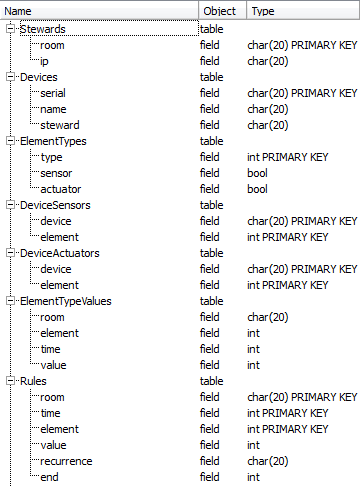
\includegraphics{database.png}
	\end{center}
	\caption{Het database schema}
\end{figure}

\subsection{Overview}

\subsubsection{Class}
\begin{description}
	\item[\hyperlink{manager}{manager}] : Een database manager.
\end{description}

\newpage
\hypertarget{manager}{\subsection{manager}}
Een database manager. Deze laat toe om devices en stewards gemakkelijk op te slagen, en een central-unit te krijgen gebaseerd op de gegevens van de database.

\subsubsection{Constructor}
\begin{description}
	\item[\hyperlink{manager:new-db-manager}{\racket{\lb[new-db-manager]\rb \ar \code{procedure?}}}] : Maakt een nieuwe manager aan.
\end{description}

\subsubsection{Method}
\begin{description}
	\item[\hyperlink{manager:add-device}{\racket{\lb[add-device] device\rb \ar \code{void?}}}] : Voegt een device toe aan de database.
	\item[\hyperlink{manager:add-steward}{\racket{\lb[add-steward] steward\rb \ar \code{void?}}}] : Voegt een steward toe aan de database.
	\item[\hyperlink{manager:restore-state}{\racket{\lb[restore-state]\rb \ar \code{central-unit?}}}] : Geeft een central-unit terug die stewards beheert die opgeslagen waren in de database.
\end{description}

\begin{framed}
	\hypertarget{manager:new-db-manager}{\racket{\lb[new-db-manager]\rb \ar \code{procedure?}}}
	\\Maakt een nieuwe manager aan.
\end{framed}

\begin{framed}
	\hypertarget{manager:add-device}{\racket{\lb[add-device] device\rb \ar \code{void?}}}
	\\Voegt een device toe aan de database. Pas op, als de device al door een steward beheert is zal de gegevensbank proberen om die nogmaals op te slagen bij het saven van de steward.
	\begin{itemize}
		\item \emph{device} : De device dat toegevoegd wordt aan de database.
	\end{itemize}
\end{framed}

\begin{framed}
	\hypertarget{manager:add-steward}{\racket{\lb[add-steward] steward\rb \ar \code{void?}}}
	\\Voegt een steward toe aan de database. Alle devices die deze steward beheert worden ook aan de gegevensbank toegevoegd.
	\begin{itemize}
		\item \emph{steward} : De steward dat toegevoegd wordt aand de database.
	\end{itemize}
\end{framed}

\begin{framed}
	\hypertarget{manager:restore-state}{\racket{\lb[restore-state]\rb \ar \code{central-unit?}}}
	\\Geeft een central-unit terug die stewards beheert die opgeslagen waren in de database.
	\begin{itemize}
		\item \emph{return} : Een central-unit die de stewards en devices beheert die in de gegevensbank opgeslagen waren.
	\end{itemize}
\end{framed}

\newpage
\hypertarget{unit-test}{\section{unit-test}}
Bevat een aantal tests om te zien of de functionaliteiten van het programma goed zijn geimplementeerd. Meeste van de interne werking en communicatie wordt getest, voor de GUI is dit niet het geval.

\subsection{Overview}

\subsubsection{Class}
\begin{description}
	\item[test-element] : Een reeks tests op element.
	\item[test-sensor] : Een reeks tests op sensor.
	\item[test-actuator] : Een reeks tests op actuator.
	\item[test-device] : Een reeks tests op device.
	\item[test-steward] : Een reeks tests op steward.
	\item[test-instruction] : Een reeks tests op instruction.
	\item[test-messenger] : Een reeks tests op messenger.
	\item[test-parser] : Een reeks tests op parser.
	\item[test-hardware-device] : Een reeks tests op hardware-device.
	\item[test-physical-room] : Een reeks tests op physical-room.
\end{description}

\end{document}